%% Copernicus Publications Manuscript Preparation Template for LaTeX Submissions
%% ---------------------------------
%% This template should be used for copernicus.cls
%% The class file and some style files are bundled in the Copernicus Latex Package which can be downloaded from the different journal webpages.
%% For further assistance please contact the Copernicus Publications at: publications@copernicus.org
%% http://publications.copernicus.org


%% Please use the following documentclass and Journal Abbreviations for Discussion Papers and Final Revised Papers.


%% 2-Column Papers and Discussion Papers
\documentclass[hess, manuscript]{copernicus}
%\documentclass[hess]{copernicus}

%% Journal Abbreviations (Please use the same for Discussion Papers and Final Revised Papers)
% Hydrology and Earth System Sciences (hess)

\usepackage[utf8]{inputenc}


\begin{document}

\linenumbers

\title{The Analog Method for Precipitation Downscaling: Finding Better Analog Situations at a Sub-Daily Time Step}


\Author[1,2]{Pascal}{Horton}
\Author[3]{Charles}{Obled}
\Author[1]{Michel}{Jaboyedoff}

\affil[1]{University of Lausanne, Institute of Earth Sciences, Lausanne, Switzerland}
\affil[2]{University of Bern, Oeschger Centre for Climate Change Research, Institute of Geography, Bern, Switzerland}
\affil[3]{Universit\'{e} de Grenoble-Alpes, LTHE, Grenoble, France}



\runningtitle{Finding Better Analog Situations at a Sub-Daily Time Step}

\runningauthor{P. Horton et al.}

\correspondence{Pascal Horton (pascal.horton@alumnil.unil.ch)}



\received{}
\pubdiscuss{} %% only important for two-stage journals
\revised{}
\accepted{}
\published{}

%% These dates will be inserted by Copernicus Publications during the typesetting process.


\firstpage{1}

\maketitle



\begin{abstract}
The Analog Method (AM) aims at predicting local weather variables (predictands), such as precipitations, by means of a statistical relationship with predictors at a synoptic scale. The analogy is generally assessed in the first place on the geopotential field by mean of a comparison of the gradients, in order to sample the days with a similar atmospheric circulation. 

The search for candidate situations, for a given target day, is usually undertaken by comparing the state of the atmosphere at fixed hours of the day, for both the target day and the candidate analogs. The constraint being the use of daily time series, due to the length of available archives they provide, and the unavailability of equivalent archives at a finer time step. However, it is unlikely that the best analogy happens at the very same hour, but it may occur at a different time of the day. In order to assess the potential of finding better analogs at a different hour, a moving time window (MTW) has been introduced on a reduced archive of hourly precipitation totals.

The MTW resulted in a better analogy in terms of the atmospheric circulation, with improved values of the analogy criteria on the whole distribution of analog dates. The improvement was found to grow with the analog ranks due to an accumulation of more similar situations in the selection. Moreover, the improvement is even more important for days with heavy precipitation events, which are generally related to more dynamic atmospheric situations, where timing is more specific. 

A seasonal effect has also been identified, with larger improvements in winter than in summer, supposedly due to the stronger effect of the diurnal cycle in summer, which favors predictors at the same hour for target and analogs.

The impact of the MTW on the prediction performance has been assessed by means of a sub-daily precipitation series transformed into moving 24~h-totals at a 6-hourly time step. This resulted in an improvement of the prediction skills, which were even larger after recalibrating the AM parameters.

However, attempts to reconstruct longer precipitation series of running 24~h-totals by means of simple methods failed. It emphasized the need to use time series with an appropriate chronology. These should be available in a near future, either by means of growing observed archives, or by the establishment of precipitation reanalyses through regional modeling. Then, the use of a MTW in the AM should be considered for any application, especially when the prediction quality of extreme events is important.

\end{abstract}



\introduction  %% \introduction[modified heading if necessary]
\label{sec:introduction}

The Analog Method (AM) is based on the principle that two relatively similar synoptic situations may produce relatively similar local effects \citep{Lorenz1956, Lorenz1969}. Multiple variations of the methods exist and listings can be found in \citet{BenDaoud2016}. The versions that will be considered here are often used as references or benchmarks for various improvements.

The AM is usually implemented with a daily time step, due to the availability of long precipitation archives that have no equivalent at a finer resolution. Therefore, the analog situations are assessed on the basis of a daily time step, by comparing predictors at fixed hours of the day, otherwise one would not know what precipitation values to assign to them. However, it can be expected that the analogy of the synoptic situations does not occur systematically at the same time of the day, and that better candidates can be found by shifting to a different hour. On this assumption, a moving time window (MTW) was introduced to allow searching for candidates at different hours of the day.

Previous tests showed the benefit, in terms of analogy criteria values, of searching for analog synoptic situations at a finer time step, but without assessing the impact on the prediction skills \citep{Finet2008}. 


The MTW is explained in Sect. \ref{sec:mtw}. As this method requires sub-daily time series, the available archive length is reduced compared to more common daily measurements, which has some consequences on the performance score (Sect. \ref{sec:archive_reduction}). The benefit of introducing a MTW was assessed first in regards to the analogy criteria improvement (Sect. \ref{sec:influence_criteria}), and then in terms of precipitation prediction skill (Sect. \ref{sec:influence_scores}). Finally, the results are discussed in Sect. \ref{sec:discussion}.


%TODO: complete !!

\section{Data and methods}

\subsection{Study area and data}
\label{sec:data}

The study area is the upper Rh\^{o}ne catchment in Switzerland \cite[see also][]{Horton2012a}. Due to the low density of weather stations with high temporal resolution and long archives, no spatially aggregated rainfall was processed. The time series (on the period 1982--2007) come from 6 automatic weather stations, namely Ulrichen, Zermatt, Visp, Montana, Sion and Aigle (Fig. \ref{fig:map}), which are subject to various meteorological influences \citep{Horton2012}. The results will thereafter be presented arbitrarily for the Ulrichen station, but they are equivalent for all stations. The precipitation time series were then aggregated by means of a moving 24~h-total (see next section).

Predictors are extracted from the NCEP/NCAR reanalysis I \citep{Kalnay1996} dataset with a 6-hourly temporal resolution, 17 pressure levels, and a spatial resolution of 2.5\degree. This dataset is now relatively old, but still often used (see discussion).

\subsection{The considered analog method}
\label{sec:analog_method}

The first method is based on the analogy of the atmospheric circulation only \citep[Table \ref{table:method_2Z},][]{Obled2002, Bontron2005, Marty2012}. Searching analog situations for a target day starts by a preselection step of the potential candidate for analogy. Here, it has been limited to the 4 months centered around the target date for every year of the archive, in order to cope with seasonal effects. Then, the similarity of the atmospheric circulation of the target date with every day of the preselection is assessed by processing the \citet{Teweles1954} score ($S_{\text{TW}}$), which is a comparison of gradients, over a certain spatial window and at certain hours. The smaller the $S_{\text{TW}}$ values, the more similar the pressure fields.

The predictand, here a 24~h precipitation total, results from meteorological situations that are continuous transitions between changing circulation patterns. Thus, the observed predictors fields, extracted from reanalysis datasets, are considered at different time of the day and at different heights. In our case, the geopotential height is considered at 1000~hPa (Z1000) at 12~h~UTC and 500~hPa (Z500) at 24~h~UTC. The selection of the observation time of the predictor was found by \citet{Bontron2004} to have a significant influence.

Then, $N_{1}$ dates with the lowest values of $S_{\text{TW}}$ are considered as analogs to the target day, $N_{1}$ being a parameter to calibrate. Then, the daily observed precipitation amount of the corresponding dates provide the empirical conditional distribution considered as the probabilistic prediction for the target day. This method will be named 2Z further on.

The second reference method adds a subsequent level of analogy on moisture variables, compared by means of the root-mean-square error ($E_{\text{RMS}}$) (method 2Z-2MI, Table \ref{table:method_2Z-2MI}). This second predictor is a moisture index made of the product of the total precipitable water (TPW) with the relative humidity at 850~hPa (RH850) \citep{Bontron2004}. When adding a second level of analogy, $N_{2}$ dates are subsampled in the $N_{1}$ analogs on the atmospheric circulation, to end up with a smaller number of analog situations. When a second level of analogy is added, a higher number of $N_{1}$ analogs is kept on the first level.


\subsection{Calibration of the analog method}
\label{sec:calibration}

To calibrate the method, the commonly used technique is a semi-automatic sequential procedure elaborated by \citet{Bontron2004}.




\subsection{The moving time window (MTW) approach}
\label{sec:mtw}

In order to assess the benefit of searching analog situations at a sub-daily time step, an appropriate precipitation series is required. On the basis of high resolution time series (Sect. \ref{sec:data}), 24~h-totals were processed, but at a 6-hourly time step (temporal resolution of the reanalysis dataset), by means of a moving 24~h-total. 

The target situations and their corresponding observed precipitation values (used for validation) do not change, because the prediction is always established for a fixed period of the target day (6--30~h), as before. The difference is that the candidates are 4~times more numerous (Fig. \ref{fig:principle}).

Based on some preliminary tests (not shown), no constraint was added in order to restrict the selection of multiple analogs within the same candidate dates.



In order to assess this potential improvement of the prediction, precipitation data with a resolution of 10 minutes, on a respectable archive length, was used (Sect. \ref{sec:data}). It was then aggregated in the form of 24~h-totals, but starting at different 6-hourly time step, by means of a moving total.



\subsection{Performance score}
\label{sec:performance}

The score that is most often considered to assess an AM performance is the Continuous Ranked Probability Score \citep[$S_{\text{CRP}}$,][]{Brown1974, Matheson1976, Hersbach2000}. It allows evaluating the predicted cumulative distribution functions $F(y)$, for example of the precipitation values $y$ from analog situations, compared to the observed value $y^{0}$. The better the prediction, the smaller the score. It is defined as follows:

\begin{equation}
\label{eq:CRPS}
S_{\text{CRP}} = \int_{-\infty}^{+\infty} \left[ F(y)-\text{H}(y-y^{0})\right]^{2} \text{d}y ,  
\end{equation}
where $\text{H}(y-y^{0})$ is the Heaviside function that is null when $y-y^{0}<0$, and has the value 1 otherwise.

In order to compare the value of the score in regard to a reference, one often considers its skill score expression, and use the climatological distribution as the reference. The Continuous Ranked Probability Skill Score ($S_{\text{SCRP}}$) is thus defined as following:

\begin{equation}
\label{eq:CRPSS}
S_{\text{SCRP}} = \frac{S_{\text{CRP}}-S_{\text{CRP}}^{r}}{S_{\text{CRP}}^{p}-S_{\text{CRP}}^{r}} = 1-\frac{S_{\text{CRP}}}{S_{\text{CRP}}^{r}}
\end{equation}
where $S_{\text{CRP}}^{r}$ is the $S_{\text{CRP}}$ value for the reference (climatological distribution) and $S_{\text{CRP}}^{p}$ would be the one for a perfect prediction (which implies $S_{\text{CRP}}^{p}~=~0$). A better prediction is characterized by an increase in $S_{\text{SCRP}}$. 



Finding better analog situations does not obligatory imply better skills to predict the precipitation. Therefore, the impact of the MTW introduction, and thus the selection of other analog dates, has to be assessed on the performance scores. In order to perform this assessment, the 24~h-totals (moving average) at a 6-hourly time step were used (see Sect. \ref{sec:data}). The target dates remain unchanged, since the original time slot (6~h~UTC -- 6~h~UTC the next day) is kept, and thus the performance scores can be directly compared with the former ones.



\section{Results}


\subsection{Consequences of the archive reduction}
\label{sec:archive_reduction}

As sub-daily precipitation time series are usually available on a shorter period than traditional daily time steps, the first assessment consists in assessing the loss of performance resulting from a reduction of a 47~years archive (1961 to 2008) to 25~years (1982 to 2007). This change is assessed with the original method, without MTW.

Both 2Z (Table \ref{table:method_2Z}) and 2Z-2MI (Table \ref{table:method_2Z-2MI}) methods were considered. The AM parameters were calibrated on the original archive (Tables \ref{table:performance}) and will be used thereafter.

The impact of the change in the archive length is summarized in Table \ref{table:loss_reduction} for both 2Z and 2Z-2MI methods. As expected, a loss of performance can be observed for each station, except for that of Aigle, which seems relatively indifferent to this change. This loss is globally significant, with up to -1.89 points for Visp and the 2Z method. 


\subsection{Influence on the analogy criteria}
\label{sec:influence_criteria}

\subsubsection{Changes in the atmospheric circulation analogy}

When searching for analogs on the geopotential heights, as in the 2Z method, there are now 4 times more candidates than before, which obviously allows to find better matches.

Figure \ref{fig:changes_S1_analogs} presents the changes in the distributions of the $S_{\text{TW}}$ criterion for the $1^{st}$, $5^{th}$, $20^{th}$ and $40^{th}$ analogs for the Ulrichen station on the whole calibration period, due to introduction of the MTW. The precipitation target remains as before, that is centered on 18~h~UTC (6~h~UTC to 6~h~UTC the next day). The shapes of the distributions of the conventional approach and the MTW are similar, but the values of the analogy criteria are now reduced (shifted to the left), and therefore better. An increase in the difference between a fixed window and a moving window is identifiable, which means that the last analogs are further improved. The latter effect is due to the accumulation of improvements brought by the new analog situations in the selection.

The improvements of the $S_{\text{TW}}$ criteria are summarized in Fig. \ref{fig:changes_S1}, which shows (top) quantiles of the $S_{\text{TW}}$ criteria according to the analog rank for the conventional method and the MTW, and (bottom) quantiles of the relative reduction. This confirms that all quantile seem similarly reduced ($S_{\text{TW}}$ distributions keep their shape), and that this improvement is constantly increasing from the first to the last analog (Fig. \ref{fig:changes_S1} bottom).


\subsubsection{Changes per precipitation classes}
\label{sec:influence_precip}

The impact of the MTW on the analogy criteria has been decomposed per precipitation classes. The results of this analysis are summarized in Fig. \ref{fig:changes_S1_precip_threshold} by the median reduction of $S_{\text{TW}}$ for days with precipitation (organized into classes) between two thresholds. The number of cases per class being reduced, the curves are not as smooth as in previous analyzes. It is nevertheless clear that the improvement tends to increase on days with higher precipitation. This is true for all our stations.


\subsubsection{Changes per season}
\label{sec:seasonal_effect}

Atmospheric dynamics varies greatly from one season to another, which reflects on the performance of the AM that is generally lower between June and August \citep{Bliefernicht2010}. It therefore makes sense to verify the effect of the MTW separately per season.

A seasonal effect can be observed on the reduction of the $S_{\text{TW}}$ criteria due to the MTW (Fig. \ref{fig:changes_S1_seasons}). The improvements are greater for winter than summer. 


\subsubsection{Changes in the moisture analogy}

When considering the second level of analogy of the 2Z-2MI method (Table \ref{table:method_2Z-2MI}), the number of candidates situations did not increase, as they are subsampled in the previously $N_{1}$ selected analogs, but their dates have changed. In contrast to earlier, both a reduction or an increase of the $E_{\text{RMS}}$ analogy criterion values are possible. Indeed, Fig. \ref{fig:changes_RMSE} shows an almost insignificant improvement of the $E_{\text{RMS}}$ values. Unlike for the first level of analogy, the relative improvement of the $E_{\text{RMS}}$ values are distributed relatively symmetrically around zero, with improvements and losses of the same amplitude. Once again, the results for the other stations are similar.


\subsection{Impact on performance scores}
\label{sec:influence_scores}

A systematic improvement of the $S_{\text{TW}}$ values was previously observed. 

The new performance scores are provided in Table \ref{table:CRPSS_MTW}, along with the differences regarding the conventional method with the same archive length. The differences ranges from 0.57 to 2.14 points for the 2Z method and from 1.53 to 2.20 points for the 2Z-2MI method. The introduction of the MTW brings an improvement of the performance that is not very large, but that is nevertheless significant. Moreover, it requires no additional predictor. No relationship was found between the improvement of the score and the reduction of the $S_{\text{TW}}$ criteria, neither with the season.


\subsubsection{Improvement per precipitation classes}
\label{sec:improvement_CRPSS_precip_threshold}

The $S_{\text{TW}}$ criteria was previously found to be improved to a greater extent for the most dynamic situations related with higher precipitation values (Sect. \ref{sec:influence_precip}). The changes in terms of performance scores will now be assessed regarding precipitation thresholds. Fig. \ref{fig:changes_CRPS_precip_threshold} synthesizes these differences for the Ulrichen station, other stations having the same behavior.

The increasing positive trend of skill improvements regarding the precipitation threshold is significant and shows that the prediction of higher precipitation totals is further improved. Thus, both the analogy criteria and the performance scores are improved to a greater extent for heavier precipitation events. On the contrary, the non-rainy days and small accumulations are not improved.


\subsubsection{Recalibration of the AM parameters}
\label{sec:recalibration}

The previous assessment of the performance improvement was established with the original parameters optimized with a fixed time window. However, one can assume that the introduction of the MTW may change the optimum of some parameters. The calibration has then been reprocessed.

After recalibrating, some changes in the optimal number of analogs can be observed for both 2Z and 2Z-2MI methods (Table \ref{table:nb_analogs_new}). Among these, the east-west dimension of the spatial windows of the circulation analogy tends to decrease (not shown). More significantly, the optimal number of analogs increases after introducing the MTW, of a significant order of magnitude: 25~\% to 83~\% for the 2Z method and 20~\% 67~\% for the 2Z-2MI method. The number of analogs of the first analogy level of the 2Z-2MI method even reached three times its previous value for the Visp station. 

This increase in number of analogs has a slight effect on the performance of the different precipitation classes. The same analysis as in Sect. \ref{sec:improvement_CRPSS_precip_threshold} has been performed again on the basis of the newly calibrated parameters. The results are generally very similar, but a slight performance increase of small precipitation values can be observed at the expense of higher amounts. The change in the analogs numbers is likely to be responsible for this difference in the performance distributions.

The values of the $S_{\text{SCRP}}$ scores for both methods (Table \ref{table:CRPSS_recalibration}) have significantly increased after recalibration. 


\section{Discussion}
\label{sec:discussion}


\subsection{Improvement of the atmospheric circulation analogy}

The median of the $S_{\text{TW}}$ values reduction (Fig. \ref{fig:changes_S1} bottom) starts approximately at 5~\% for the first analog and reaches more than 10~\% for the last one. This increasing trend with the analog rank can be explained by the accumulation of better analogs in the distribution. The minimum improvement starts from 0 and reaches 2--3\%, meaning that the criteria have been improved on most analogs for every day of the calibration period. All other stations have a similar improvement of the $S_{\text{TW}}$ criteria, both in terms of distribution shape and amplitude.

\subsection{Improvement of the moisture analogy}




This result of a globally null improvement of the $E_{\text{RMS}}$ values does not mean that the 2Z-2MI method cannot be improved by the MTW. It means that after the selection of the analogs situations in terms of the synoptic circulation, the new candidate dates do not allow to find better analogs in terms of moisture. However, the selected dates have changed in the first level of analogy, and thus also in the final selection, which can potentially improve the performance scores on the predictand.




With the introduction of the MTW, the performance loss related to the reduction of the archive length is compensated.



\subsection{Impact of the MTW per precipitation classes}




It can be assumed that the atmospheric conditions with a low dynamism, such as the frequent anticyclonic situations, will not be radically improved by the introduction of the MTW. Conversely, dynamic situations, such as weather disturbances, have a well marked temporal evolution. Indeed, the position of the driving elements such as the low-pressure center and the fronts change significantly during a day. We can therefore expect to improve more significantly these situations with a higher dynamism when introducing a MTW, as better matches to the target situation may be found.

The dynamism of a given atmospheric condition cannot be easily quantified. A basic assumption is considered here, which stipulates that the more a day is rainy, the more dynamic the situation is. 




\subsection{Seasonal effect}


One hypothesis is that the diurnal effects of the summer months have an influence on the atmospheric circulation, at least in the lower layers. This effect is based on the daily cycle and good analogs are essentially found for the same hours or time windows.

An analysis of the selected hours for the geopotential predictor seems to confirm this assumption (Fig. \ref{fig:hours_selection_per_season}). It was found that the new choice of the temporal window in winter, when using the MTW approach, is well balanced between the 4 options. This means a change of 75\% of the analogs selection compared to the conventional approach, which improves the circulation analogy.

On the contrary, the summer months have a preference for the initial temporal window (Z500 24~h \& Z1000 12~h), due to more pronounced diurnal effects which reduces the potential for improvement of the criteria. Other seasons are between these two extremes, which is consistent with their respective improvements. This seasonal effect was observed for each station in a very similar way, and generally even with a slightly larger amplitude than for Ulrichen (see example of the Visp station in Fig. \ref{fig:hours_selection_per_season_Visp}).

\subsection{Increase in number of analog situations}



It seems as if the method perceive the increase in the archive length and diversity by allowing to extract more analogs. As we saw in Fig. \ref{fig:changes_S1}, the improvement of the $S_{\text{TW}}$ criteria grows along with the rank of the analog, which shows an accumulation of better analog situations in the distributions. It seems thus profitable to widen the selection of analogs in order to keep also some whose rank has increased, as they appear to be also relevant to predict precipitation values. The number of good analogs is thus globally increased.




\subsection{Why not just making a 6-hourly prediction ?}

One can question the interest of using daily totals when a 6-hourly precipitation series can be used. The first reason is that the 6-hourly time series generated by the AM may not represent well the dynamic of the accurate precipitation (results not shown), due to a smoothed signal. Then, sometimes one just does not need finer resolution than the daily time step. Finally, when using a reconstructed precipitation archive, the errors in intra-day precipitation distributions have a lesser impact over 24~h daily totals.

\subsection{On the use of an old reanalysis dataset}

The considered reanalysis dataset, which is the NCEP/NCAR reanalysis I \citep{Kalnay1996}, is relatively old and has a coarse resolution. Newer reanalysis dataset could have been used to achieve this study, and might have resulted in higher performance scores. However, one can assume that the gain observed here by introducing a MTW should also be found for a better reanalysis dataset, especially if the information of the atmospheric circulation is more accurate.

\subsection{Is a simple reconstructed archive useful for the MTW ?}

The improvement provided by the MTW is interesting, mainly for heavy precipitation events, and thus it would be profitable to be able to apply it to the complete archive. Unfortunately, there is no long precipitation time series available with a sub-daily time step. In order to reconstruct a longer archive of moving 24~h-totals, different disaggregation approaches of the daily time series were assessed.

A proportional distribution is certainly the simplest approach that can be performed. It consists in allocating proportional parts of the original daily time series into a new moving average of 24~h-totals (Fig. \ref{fig:illustration_disaggregation}). When using this reconstructed time series on the shorter period, the method performance was degraded (Table \ref{table:disaggregation_proportional} to compare to Table \ref{table:CRPSS_MTW}) and was even below the conventional method without MTW (Table \ref{table:loss_reduction}). The benefit of a better selection of the analog situations is lost due to a precipitation archive of poor quality.

\subsection{Can a proxy variable help reconstruct a better archive ?}

As demonstrated in the previous section, the performance improvement brought by the MTW is lost when using a simplistic precipitation time series. In order to get closer to the chronology of the actual precipitation, the reconstruction procedure must rely on some informative variable. Data from the NCEP/NCAR reanalysis 1 (Sect. \ref{sec:data}) was used in this perspective, despite their rough resolution.

The best proxy variable was identified by means of a correlation analyses (on non-zero values) with the 6-hourly precipitation time series on the period 1982-2007. Precipitable water and relative humidity (at 1000~hPa, 925~hPa or 850~hPa) were assessed at the four points surrounding the catchment, and by allowing a time lapse between both series in order to take into account the significant distance separating the weather stations and the reanalysis grid point (details not shown). The best proxy for the Zermatt station is the precipitable water at 45° N and 7.5° E, with a time offset of -6~h.

Table \ref{table:proxy_CRPSS} presents the $S_{\text{SCRP}}$ scores obtained by the reconstituted series using the proxy of precipitable water. A slight improvement can be obtained compared to the proportional distribution method, but it is still relatively small, and most of the benefit of the MTW is again lost. A more recent reanalysis archive with more accurate moisture variables might produce better proxies.

These attempts to transpose the MTW on the total archive highlight the importance of the actual rainfall chronology. The MTW is profitable, provided that the precipitation series are close to the observed one. Without precipitation series with an accurate sub-daily chronology, the introduction of a MTW remains fruitless.



\conclusions  %% \conclusions[modified heading if necessary]

The AM is most often based on a daily time step, due to the availability of long precipitation archives. However, it is unlikely that two analog synoptic situations, that evolve relatively quickly, would correspond optimally at the same hour of the day. It is thus more likely that a better match can be found at another time, which can change the selection of the analogs dates.

As \citet{Finet2008} had previously shown, the introduction of a MTW allows finding better analog situations in terms of the atmospheric circulation. It has been here demonstrated that the improvement of the $S_{\text{TW}}$ criteria values is growing with the rank of the analog. This is due to the accumulation of better analogs within the predicted distributions.

The improvement of the circulation analogy was found to be more important for heavy precipitation events, which are generally related to more dynamic atmospheric situations. This dynamism implies more specific circulation patterns that are evolving more rapidly. Thus, a MTW is found to be of particular interest in this kind of situation, and benefits the prediction of extreme precipitation events.

A seasonal effect has been highlighted, as the MTW is more profitable for winter months than summer. The reason is likely that the diurnal cycle has a bigger effect in summer than in winter, which results in better analogs at the same time of the day. The preference for the same hours in summer has been demonstrated, whereas 75\% of the analog situations are selected at a different time in winter.

The impact of the MTW on the prediction performance has never been assessed before, due to the shortcoming of long precipitation series at a sub-daily time step. The impact of the MTW approach could be assessed on a 25 years time series with a high temporal resolution. After the introduction of the MTW, the performance scores increased of the same order of magnitude as if the length of the archive doubled, in this case study.

The parameters were then calibrated again, using the MTW. Some parameters changed, the main difference being the number of analogs, which systematically and significantly increased compared to the original set. A wider selection of analog situations, containing those whose rank decreased, seemed profitable for the prediction performance. The number of good analogs is thus globally increased. This change seems to benefit mainly the prediction of days with small precipitation totals.

The importance of the quality of the precipitation archive was also demonstrated, as too simplistic reconstructions of 6-hourly time series lead to a loss of all the improvement brought by better analog situations identified by the MTW. The precipitation prediction is improved only when the precipitation chronology is close to the accurate one. Attempts to reconstruct longer time series based on a simplistic proportional distribution or using meteorological variables from the NCEP reanalysis 1 dataset as proxy did not succeed. Other reanalysis datasets could eventually preform better.

Perspectives of using the MTW rely on the availability of long precipitation series at a sub-daily time step and with high accuracy. The first source of such data is the simple fact that with time, these archives of high temporal resolution precipitation data are getting longer. The second source is the establishment of precipitation reanalysis at a country scale, or the use of reanalysis-driven RCMs (Regional Climate Models) or LAMs (Limited Area Models) on a long period. When such precipitation data will be available, the use of a MTW in the AM should be considered for any application, especially when the prediction quality of extreme events is important.



\begin{acknowledgements}
Thanks to Dominique B\'{e}rod for his support and to Renaud Marty for his fruitful collaboration over the years. 

Thanks to the Swiss Federal Office for Environment (FOEV), the Roads and Water courses Service, Energy and Water Power Service of the Wallis Canton and the Water, Land and Sanitation Service of the Vaud Canton who financed the MINERVE (Mod\'{e}lisation des Intemp\'{e}ries de Nature Extr\^{e}me des Rivi\`{e}res Valaisannes et de leurs Effets) project which started this research. 

The fruitful collaboration with the Laboratoire d'Etude des Transferts en Hydrologie et Environnement of the Grenoble Institute of Technology (G-INP) was made possible thanks to the Herbette Foundation. 

NCEP reanalysis data provided by the NOAA/OAR/ESRL PSD, Boulder, Colorado, USA, from their Web site at http://www.esrl.noaa.gov/psd/. Precipitation time series provided by MeteoSwiss. 
\end{acknowledgements}


%% REFERENCES

%% The reference list is compiled as follows:

\bibliographystyle{copernicus}
\bibliography{../_refs/4_articles-2016_HESS_moving-window}




\begin{figure}[htb]
	\begin{center}
		\includegraphics[width=8.3cm]{figures/figure_map.pdf}
	\end{center}
	\caption{Position of the 6 weather stations of interest (Ulrichen, Zermatt, Visp, Montana, Sion and Aigle) in the study area.}
	\label{fig:map}
\end{figure}

\begin{figure}[htb]
	\begin{center}
		
\includegraphics[width=8.3cm]{figures/illustration_moving_window.pdf}
	\end{center}
	\caption{Illustration of the principle of a moving time window. The larger horizontal bars represent the 24~h precipitation totals.}
	\label{fig:principle}
\end{figure}

\begin{figure*}[htb]
	\begin{center}
		\includegraphics[width=15cm]{figures/changes_S1_analogues.pdf}
	\end{center}
	\caption{Changes in the $S_{\text{TW}}$ criteria distributions of (a) the $1^{st}$, (b) $5^{th}$, (c) $20^{th}$ and (d) $40^{th}$ analog ranks for the Ulrichen station, due to the MTW.}
	\label{fig:changes_S1_analogs}
\end{figure*}

\begin{figure}[htb]
	\begin{center}
		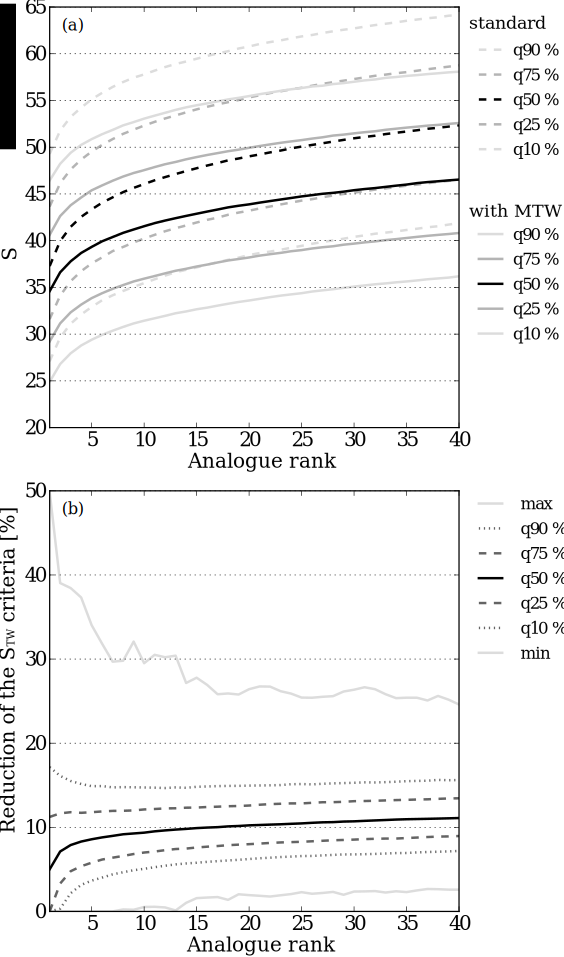
\includegraphics[width=8.2cm]{figures/changes_S1_value_and_gain.pdf}
	\end{center}
	\caption{Synthesis of the changes in the $S_{\text{TW}}$ criteria, due to the MTW, for the Ulrichen station, depending on the ranks of the analog. (a) Quantiles of the $S_{\text{TW}}$ distributions with and without the MTW. (b) Quantiles of the relative improvements of the S1 criteria when using the MTW.}
	\label{fig:changes_S1}
\end{figure}

\begin{figure}[htb]
	\begin{center}
		\includegraphics[width=8.3cm]{figures/changes_S1_precip_threshold.pdf}
	\end{center}
	\caption{Distribution of the median improvements of the $S_{\text{TW}}$ criteria, due to the MTW, depending on precipitation thresholds at the Ulrichen station.}
	\label{fig:changes_S1_precip_threshold}
\end{figure}

\begin{figure}[htb]
	\begin{center}
		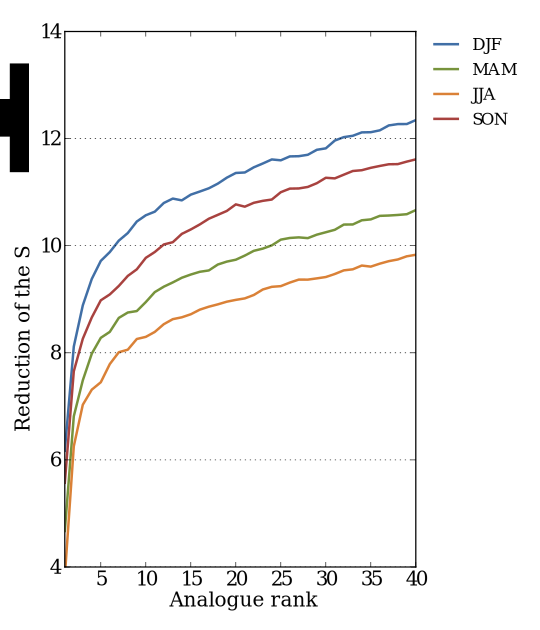
\includegraphics[width=7cm]{figures/changes_S1_seasons.pdf}
	\end{center}
	\caption{Seasonal effect on the median reduction of the $S_{\text{TW}}$ criteria for the Ulrichen station due to the MTW. DJF: winter, MAM: spring, JJA: summer SON: fall.}
	\label{fig:changes_S1_seasons}
\end{figure}

\begin{figure}[htb]
	\includegraphics[width=8.3cm]{figures/hours_selection_per_season.pdf}
	\caption{Distribution of the predictors hours in the selected analog dates depending on the season, for the Ulrichen station.}
	\label{fig:hours_selection_per_season}
\end{figure}

\begin{figure}[htb]
	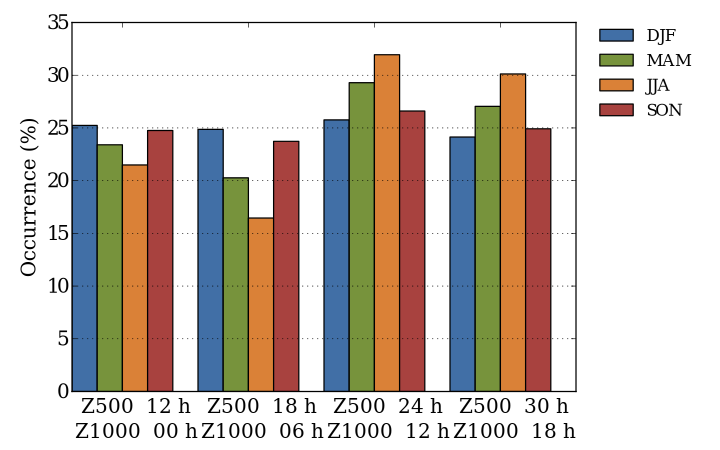
\includegraphics[width=8.3cm]{figures/hours_selection_per_season_Visp.pdf}
	\caption{Distribution of the predictors hours in the selected analog dates depending on the season, for the Visp station.}
	\label{fig:hours_selection_per_season_Visp}
\end{figure}

\begin{figure}[htb]
	\begin{center}
		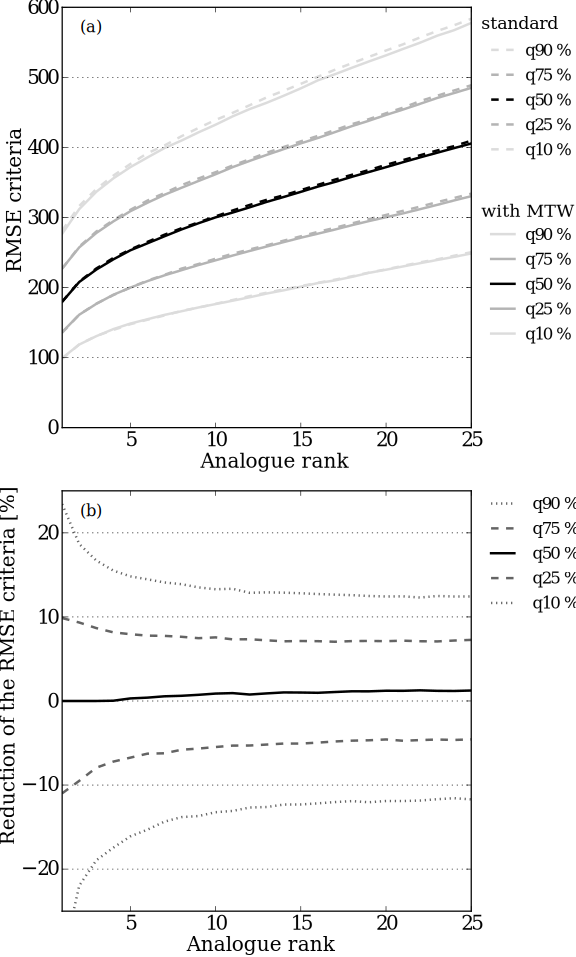
\includegraphics[width=8.1cm]{figures/changes_RMSE_value_and_gain.pdf}
	\end{center}
	\caption{Synthesis of the changes in the $E_{\text{RMS}}$ criteria, due to the MTW, for the Ulrichen station, depending on the ranks of the analog. (a) Quantiles of the $E_{\text{RMS}}$ distributions with and without the MTW. (b) Quantiles of the relative improvements of the $E_{\text{RMS}}$ criteria when using the MTW.}
	\label{fig:changes_RMSE}
\end{figure}

\begin{figure}[htb]
	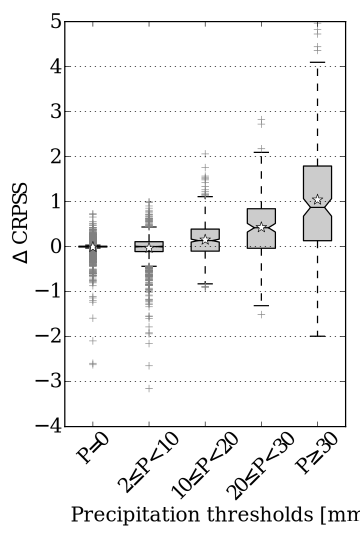
\includegraphics[width=5cm]{figures/changes_CRPS_precip_threshold.pdf}
	\caption{Differences of the $S_{\text{SCRP}}$ performance score, due to the introduction of the MTW, as a function of precipitation thresholds at the Ulrichen station. The stars represent averages.}
	\label{fig:changes_CRPS_precip_threshold}
\end{figure}

\begin{figure}[htb]
	\begin{center}
		\includegraphics[width=8cm]{figures/illustration_disaggregation.pdf}
	\end{center}
	\caption{Illustration of the generation of 24~h-totals moving averages by means of a proportional distribution. The colours refer to the corresponding day of the daily time series.}
	\label{fig:illustration_disaggregation}
\end{figure}


\clearpage


\begin{table}[htb]
	\caption{Parameters of the reference method on the atmospheric circulation (2Z). The first column is the level of analogy (0 for preselection), then comes the meteorological variable and its hour of observation (temporal window). The criteria used for the current level of analogy is then provided, as well as the number of analogs.}
	\footnotesize
	\begin{center}
		\begin{tabular}{ccccc}
			\hline
			Level & Variable & Hour & Criteria & Nb \\ 
			\hline 
			0 & \multicolumn{4}{l}{$\pm 60$ days around the target date} \\
			\hline 
			\multirow{2}{*}{1} & Z1000 & 12~h & \multirow{2}{*}{$S_{\text{TW}}$} & \multirow{2}{*}{$N_{1}$} \\
			& Z500 & 24~h & & \\ 
			\hline 
		\end{tabular} 
	\end{center}
	\label{table:method_2Z}
\end{table}

\begin{table}[htb]
	\caption{Parameters of the reference method with moisture variables (2Z-2MI). Same conventions as Table \ref{table:method_2Z}}
	\footnotesize
	\begin{center}
		\begin{tabular}{ccccc}
			\hline 
			Level & Variable & Hour & Criteria & Nb \\ 
			\hline 
			0 & \multicolumn{4}{l}{$\pm 60$ days around the target date} \\
			\hline 
			\multirow{2}{*}{1} & Z1000 & 12~h & \multirow{2}{*}{$S_{\text{TW}}$} & \multirow{2}{*}{$N_{1}$} \\
			& Z500 & 24~h & & \\ 
			\hline
			\multirow{2}{*}{2} & TPW * RH850 & 12~h & \multirow{2}{*}{$E_{\text{RMS}}$} & \multirow{2}{*}{$N_{2}$} \\
			& TPW * RH850 & 24~h & & \\ 
			\hline 
		\end{tabular} 
	\end{center}
	\label{table:method_2Z-2MI}
\end{table}

\begin{table}[htb]
	\caption{Number of analogs (of the first and the second level of analogy, respectively $N_{1}$ and $N_{2}$) and skill score (\%) of the method based on the atmospheric circulation only (method 2Z), and the one with a second level of analogy on moisture variables (2Z-2MI), on the full archive.}
	\begin{center}
		\begin{tabular}{l c c c c c }
			\hline
			\multirow{2}{*}{Station} & \multicolumn{2}{c}{2Z} & \multicolumn{3}{c}{2Z-2MI} \\
			& $N_{1}$ & $S_{\text{SCRP}}$ & $N_{1}$ & $N_{2}$ & $S_{\text{SCRP}}$ \\ 
			\hline
			Ulrichen & 40 & 30.73 & 60 & 25 & 34.31 \\
			Zermatt & 35 & 23.87 & 55 & 25 & 28.28 \\
			Visp & 30 & 25.11 & 45 & 25 & 28.85 \\
			Montana & 40 & 32.55 & 55 & 30 & 36.11 \\
			Sion & 40 & 26.23 & 90 & 30 & 31.16 \\
			Aigle & 50 & 30.59 & 100 & 35 & 35.82 \\ 
			\hline
		\end{tabular}
	\end{center}	
	\label{table:performance}
\end{table}

\begin{table}[htb]
	\caption{Influence of the archive reduction on the $S_{\text{SCRP}}$. $S_{\text{SCRP}}$ values are provided for both considered methods and the differences are expressed in absolute value.}
	\begin{center}
		\begin{tabular}{l c c c c }
			\hline
			\multirow{2}{*}{Station} & \multicolumn{2}{c}{2Z} & \multicolumn{2}{c}{2Z-2MI} \\
			& 82-07 & $\Delta$ & 82-07 & $\Delta$ \\ 
			\hline
			Ulrichen & 29.37 & -1.36 & 33.24 & -1.08 \\
			Zermatt & 22.20 & -1.67 & 26.95 & -1.32 \\
			Visp & 23.23 & -1.89 & 27.77 & -1.08 \\
			Montana & 30.79 & -1.76 & 34.77 & -1.34 \\
			Sion & 24.78 & -1.45 & 29.36 & -1.80 \\
			Aigle & 30.57 & -0.01 & 35.95 & 0.13 \\ 
			\hline
		\end{tabular}
	\end{center}
	\label{table:loss_reduction}
\end{table}

\begin{table}[htb]
	\caption{New $S_{\text{SCRP}}$ performance scores for both 2Z and 2Z-2MI methods obtained by the MTW approach. The differences are expressed regarding the conventional method with the same archive length.}
	\begin{center}
		\begin{tabular}{l c c c c}
			\hline
			\multirow{2}{*}{Station} & \multicolumn{2}{c}{2Z} & \multicolumn{ 2}{c}{2Z-2MI} \\
			& MTW & $\Delta$ & MTW & $\Delta$ \\
			\hline
			Ulrichen & 31.12 & 1.74 & 35.44 & 2.20 \\
			Zermatt & 24.34 & 2.14 & 28.92 & 1.97 \\
			Visp & 24.39 & 1.16 & 29.42 & 1.64 \\
			Montana & 31.59 & 0.80 & 36.30 & 1.53 \\
			Sion & 25.35 & 0.57 & 31.07 & 1.71 \\
			Aigle & 31.78 & 1.21 & 38.11 & 2.16 \\ 
			\hline
		\end{tabular}
	\end{center}
	\label{table:CRPSS_MTW}
\end{table}

\begin{table}[htb]
	\caption{Number of analogs (of the first and the second level of analogy, respectively $N_{1}$ and $N_{2}$) of the method based on the atmospheric circulation only (method 2Z), and the one with a second level of analogy on moisture variables (2Z-2MI), using the MTW approach.}
	\begin{center}
		\begin{tabular}{l c c c }
			\hline
			\multirow{2}{*}{Station} & \multicolumn{1}{c}{2Z} & \multicolumn{2}{c}{2Z-2MI} \\
			& $N_{1}$ & $N_{1}$ & $N_{2}$ \\ 
			\hline
			Ulrichen & 50 & 110 & 35 \\
			Zermatt & 55 & 80 & 30 \\
			Visp & 55 & 135 & 35 \\
			Montana & 55 & 110 & 40 \\
			Sion & 55 & 140 & 50 \\
			Aigle & 75 & 135 & 45 \\ 
			\hline
		\end{tabular}
	\end{center}	
	\label{table:nb_analogs_new}
\end{table}

\begin{table}[htb]
	\caption{Values of the $S_{\text{SCRP}}$ (\%) skill score for the newly calibrated parameters using the MTW approach. The differences are expressed regarding the conventional method with the same archive length.}
	\begin{center}
		\begin{tabular}{l c c c c}
			\hline
			\multirow{2}{*}{Station} & \multicolumn{2}{c}{2Z} & \multicolumn{ 2}{c}{2Z-2MI} \\
			& MTW & $\Delta$ & MTW & $\Delta$ \\
			\hline
			Ulrichen & 31.58 & 2.20 & 35.72 & 2.48  \\
			Zermatt & 24.71 & 2.51 & 29.63 & 2.68 \\
			Visp & 25.08 & 1.85 & 30.29 & 2.52 \\
			Montana & 32.22 & 1.43 & 37.15 & 2.38 \\
			Sion & 26.07 & 1.29 & 31.68 & 2.32 \\
			Aigle & 32.21 & 1.64 & 38.50 & 2.55 \\
			\hline
		\end{tabular}
	\end{center}
	\label{table:CRPSS_recalibration}
\end{table}


\begin{table}[htb]
	\caption{Values of the $S_{\text{SCRP}}$ (\%) skill score for the original and the recalibrated parameters (with the sequential method, as described in Sect. \ref{sec:introduction}) using the MTW approach on the disaggregated precipitation time series (short period) by means of the proportional distribution.}
	\begin{center}
		\begin{tabular}{l c c c c}
			\hline
			\multirow{2}{*}{Station} & \multicolumn{2}{c}{2Z} & \multicolumn{ 2}{c}{2Z-2MI} \\
			& original & recalib. & original & recalib. \\
			\hline
			Ulrichen & 29.13 & 29.61 & 33.15 & 33.45 \\
			Zermatt & 22.17 & 22.80 & 26.72 & 27.43 \\
			Visp & 22.32 & 22.89 & 27.01 & 28.04 \\
			Montana & 29.41 & 30.24 & 33.83 & 34.55 \\
			Sion & 22.98 & 23.41 & 28.57 & 29.15 \\
			Aigle & 29.07 & 29.46 & 34.66 & 35.09 \\
			\hline
		\end{tabular}
	\end{center}
	\label{table:disaggregation_proportional}
\end{table}

\begin{table}[htb]
	\caption{Values of the $S_{\text{SCRP}}$ (\%) skill score for Zermatt, for the original and the recalibrated parameters (with the sequential method, as described in Sect. \ref{sec:introduction}) using the MTW approach on the disaggregated precipitation time series (short and long periods) by means of variables from the reanalysis.}
	\begin{center}
		\begin{tabular}{l c c c c}
			\hline
			\multirow{2}{*}{Period} & \multicolumn{2}{c}{2Z} & \multicolumn{ 2}{c}{2Z-2MI} \\
			& original & recalib. & original & recalib. \\
			\hline
			1982--2007 & 22.57 & 23.14 & 27.11 & 27.71 \\
			1961--2008 & 23.81 & 24.38 & 28.42 & 28.86 \\
			\hline
		\end{tabular}
	\end{center}
	\label{table:proxy_CRPSS}
\end{table}



%% Since the Copernicus LaTeX package includes the BibTeX style file copernicus.bst,
%% authors experienced with BibTeX only have to include the following two lines:
%%
%% \bibliographystyle{copernicus}
%% \bibliography{example.bib}
%%
%% URLs and DOIs can be entered in your BibTeX file as:
%%
%% URL = {http://www.xyz.org/~jones/idx_g.htm}
%% DOI = {10.5194/xyz}


%% LITERATURE CITATIONS
%%
%% command                        & example result
%% \citet{jones90}|               & Jones et al. (1990)
%% \citep{jones90}|               & (Jones et al., 1990)
%% \citep{jones90,jones93}|       & (Jones et al., 1990, 1993)
%% \citep[p.~32]{jones90}|        & (Jones et al., 1990, p.~32)
%% \citep[e.g.,][]{jones90}|      & (e.g., Jones et al., 1990)
%% \citep[e.g.,][p.~32]{jones90}| & (e.g., Jones et al., 1990, p.~32)
%% \citeauthor{jones90}|          & Jones et al.
%% \citeyear{jones90}|            & 1990



%% FIGURES

%% ONE-COLUMN FIGURES

%%f
%\begin{figure}[t]
%\includegraphics[width=8.3cm]{FILE NAME}
%\caption{TEXT}
%\end{figure}
%
%%% TWO-COLUMN FIGURES
%
%%f
%\begin{figure*}[t]
%\includegraphics[width=12cm]{FILE NAME}
%\caption{TEXT}
%\end{figure*}
%
%
%%% TABLES
%%%
%%% The different columns must be seperated with a & command and should
%%% end with \\ to identify the column brake.
%
%%% ONE-COLUMN TABLE
%
%%t
%\begin{table}[t]
%\caption{TEXT}
%\begin{tabular}{column = lcr}
%\tophline
%
%\middlehline
%
%\bottomhline
%\end{tabular}
%\belowtable{} % Table Footnotes
%\end{table}
%
%%% TWO-COLUMN TABLE
%
%%t
%\begin{table*}[t]
%\caption{TEXT}
%\begin{tabular}{column = lcr}
%\tophline
%
%\middlehline
%
%\bottomhline
%\end{tabular}
%\belowtable{} % Table Footnotes
%\end{table*}
%
%
%%% NUMBERING OF FIGURES AND TABLES
%%%
%%% If figures and tables must be numbered 1a, 1b, etc. the following command
%%% should be inserted before the begin{} command.
%
%\addtocounter{figure}{-1}\renewcommand{\thefigure}{\arabic{figure}a}
%
%
%%% MATHEMATICAL EXPRESSIONS
%
%%% All papers typeset by Copernicus Publications follow the math typesetting regulations
%%% given by the IUPAC Green Book (IUPAC: Quantities, Units and Symbols in Physical Chemistry,
%%% 2nd Edn., Blackwell Science, available at: http://old.iupac.org/publications/books/gbook/green_book_2ed.pdf, 1993).
%%%
%%% Physical quantities/variables are typeset in italic font (t for time, T for Temperature)
%%% Indices which are not defined are typeset in italic font (x, y, z, a, b, c)
%%% Items/objects which are defined are typeset in roman font (Car A, Car B)
%%% Descriptions/specifications which are defined by itself are typeset in roman font (abs, rel, ref, tot, net, ice)
%%% Abbreviations from 2 letters are typeset in roman font (RH, LAI)
%%% Vectors are identified in bold italic font using \vec{x}
%%% Matrices are identified in bold roman font
%%% Multiplication signs are typeset using the LaTeX commands \times (for vector products, grids, and exponential notations) or \cdot
%%% The character * should not be applied as mutliplication sign
%
%
%%% EQUATIONS
%
%%% Single-row equation
%
%\begin{equation}
%
%\end{equation}
%
%%% Multiline equation
%
%\begin{align}
%& 3 + 5 = 8\\
%& 3 + 5 = 8\\
%& 3 + 5 = 8
%\end{align}
%
%
%%% MATRICES
%
%\begin{matrix}
%x & y & z\\
%x & y & z\\
%x & y & z\\
%\end{matrix}
%
%
%%% ALGORITHM
%
%\begin{algorithm}
%\caption{…}
%\label{a1}
%\begin{algorithmic}
%…
%\end{algorithmic}
%\end{algorithm}
%
%
%%% CHEMICAL FORMULAS AND REACTIONS
%
%%% For formulas embedded in the text, please use \chem{}
%
%%% The reaction environment creates labels including the letter R, i.e. (R1), (R2), etc.
%
%\begin{reaction}
%%% \rightarrow should be used for normal (one-way) chemical reactions
%%% \rightleftharpoons should be used for equilibria
%%% \leftrightarrow should be used for resonance structures
%\end{reaction}
%
%
%%% PHYSICAL UNITS
%%%
%%% Please use \unit{} and apply the exponential notation


\end{document}
